\documentclass{mathnotes}

\name{Jacky Lee}
\notetitle{Real Analysis Notes}
\notedate{\today}

\begin{document}
\begin{center}
  \vspace*{20pt}
  \LARGE{Real Analysis Notes}
\end{center}

\section*{Rational Numbers and Bounds}

If $\frac{a}{b},\frac{c}{d}\in\QQ$, then
$$\frac{a}{b}+\frac{c}{d}=\frac{ad+bc}{bd} \hspace{50pt}
\frac{a}{b}-\frac{c}{d}=\frac{ad-bc}{bd} \hspace{50pt}
\frac{a}{b}\times\frac{c}{d}=\frac{ac}{bd} \hspace{50pt}
\frac{a}{b}\div\frac{c}{d}=\frac{ad}{bc}$$
provided that $\frac{c}{d}\neq\frac{0}{1}$.\\

\begin{note}
  Strictly speaking, we need to show that these operations are
  \define{well-defined} or that they don't depend on the choice of
  representatives from the equivalence classes.
\end{note}

\begin{defi}
  Suppose $S$ is an ordered set, and $E\subseteq S$. If there exists $\beta\in
  S$ such that $x\leq \beta$ for every $x\in E$, we say $E$ is \define{bounded
  above} and we call $\beta$ an \define{upper bound}. The terms \define{bounded
  below} and \define{lower bound} are defined similarly.
\end{defi}

\begin{defi}
  Suppose $S$ is an ordered set, $E\subseteq S$, and $E$ is bounded above.
  Suppose there exists $\alpha\in S$ such that $\alpha$ is an upper bound for
  $E$ and if $\gamma<\alpha$, then $\gamma$ is not an upper bound for $E$, then
  $\alpha$ is the \define{least upper bound} of $E$ or the \define{supremum} of
  $E$, and we write $\alpha=\sup{E}$. The \define{greatest lower bound} and
  \define{infimum} ($\inf{E}$) are defined similarly.
\end{defi}

\begin{ex}
  Consider the set $\{r\in\QQ:r^2<2\}$, which has no supremum in $\QQ$.
\end{ex}

\begin{defi}
  An ordered set $S$ has the \define{least-upper-bound property} if the
  following is true: if $E\subseteq S$, $E$ is not empty, and $E$ is bounded
  above, then $\sup{E}$ exists in $S$.
\end{defi}

\begin{prop}
  If an ordered set has the least-upper-bound property, then it also has the
  greatest-lower-bound property.
\end{prop}

\begin{defi}
  There exists an ordered field $\RR$ (called the \define{real numbers}) which
  has the least-upper-bound property, and it contains an isomorphic copy of
  $\QQ$.
\end{defi}

\begin{note}
  Finite ordered fields do not exist. Consider $0\leq1\leq1+1\leq\ldots$ which
  can't be a finite chain.
\end{note}

\section*{Dedekind Cuts}

\begin{enumerate}
  \item Define the elements of $\RR$ as subsets of $\QQ$ called \define{cuts},
    where a cut is a subset $\alpha$ of $\QQ$ such that
    \begin{enumerate}
      \item $\alpha$ is a nonempty proper subset of $\QQ$
        ($\alpha\ne\varnothing$ and $\alpha\ne\QQ$).
      \item If $p\in\alpha$, $q\in\QQ$, and $q<p$, then $q\in\alpha$.
      \item If $p\in\alpha$, then $p<r$ for some $r\in\alpha$ (can't be in the
        set and be an upper bound).
    \end{enumerate}
  \item Define an order on $\RR$ where $\alpha<\beta$ if and only if $\alpha$
    is a proper subset of $\beta$.
  \item Show that the ordered set $\RR$ has the least-upper-bound property. To
    do this, suppose $A$ is a nonempty subset of $\RR$ that is bounded above.
    Let $\gamma$ be the union of all $\alpha\in A$. Then show $\gamma\in\RR$
    and $\gamma=\sup A$.
  \item For $\alpha,\beta\in\RR$, define the sum $\alpha+\beta$ to be the set
    of all sums $r+s$ where $r\in\alpha$ and $s\in\beta$. Define
    $0^*=\{t\in\QQ:t<0\}$ then show axioms for addition in fields hold for
    $\RR$, and that $0^*$ is the additive identity.
  \item Show that if $\alpha,\beta,\gamma\in\RR$ and $\beta<\gamma$, then
    $\alpha+\beta<\alpha+\gamma$. This is part of showing that $\RR$ is an
    ordered field.
  \item For $\alpha,\beta\in\RR$, where $\alpha>0^*$ and $\beta>0^*$, define
    the product $\alpha\beta$ to be $\{p\in\QQ:q\le rs,\ r\in\alpha,\
    s\in\beta,\ r>0,\ s>0\}$. Note that $\alpha\beta>0^*$ if $\alpha>0^*$ and
    $\beta>0^*$, which is part of showing that $\RR$ is an ordered field.
  \item Extend the definition of multiplication to all of $\RR$ by setting, for
    all $\alpha,\beta\in\RR$, $\alpha0^*=0^*\alpha=0^*$ and
    $$\alpha\beta=\begin{cases}
      (-\alpha)(-\beta) & \alpha<0^*, \beta<0^*\\
      -[(-\alpha)(\beta)] & \alpha<0^*, \beta>0^*\\
      -[(\alpha)(-\beta)] & \alpha>0^*, \beta<0^*
    \end{cases}$$
    then prove the distributive law.
  \item Associate to each $r\in\QQ$ the real number $r^*=\{t\in\QQ:t<r\}$ and
    let $\QQ^*=\{r^*:r\in\QQ\}$. These are the rational cuts in $\RR$.
  \item Show that $\QQ$ is isomorphic to $\QQ^*$ as ordered fields.
\end{enumerate}

\section*{Properties of Real Numbers}

\begin{thm}
  Any two ordered fields with the least upper-bound-property are isomorphic.
\end{thm}

\begin{thm}
  If $x,y\in\RR$, and $x>0$, then there is a positive integer $n$ such that
  $nx>y$. This is called the \define{Archimedean property} of $\RR$.
\end{thm}

\begin{pf}
  Let $A=\{nx:n\in\ZZ^+\}$ and suppose the Archimedean property is false. Then
  $y$ would be an upper bound of $A$. But then $A$ would have a least upper
  bound. Say $\alpha=\sup A$. Since $x>0$, $\alpha-x<\alpha$, and $\alpha-x$ is
  not an upper bound. Thus, $\alpha-x<mx$ for some $m\in\ZZ^+$. But then
  $\alpha<(m+1)x$, which contradicts the fact that $\alpha$ is an upper bound
  of $A$. Thus, the Archimedean property must be true.
\end{pf}

\begin{thm}
  If $x,y\in\RR$ and $x<y$, then there exists $p\in\QQ$ such that $x<p<y$. We
  say that $\QQ$ is \define{dense} in $\RR$.
\end{thm}

\begin{thm}
  For every positive real number $x$ and every positive integer $n$, there is
  exactly one positive real number $y$ such that $y^n=x$.
\end{thm}

\begin{pf}
  There is at most one since $0<y_1<y_2$ implies $y_1^n<y_2^n$. Let
  $E=\{t\in\RR:t>0,t^n<x\}$. Then $E$ is nonempty since
  $t=\frac{x}{1+x}\implies0<t<1\implies t^n<t<x\implies t\in E$. We also know
  $E$ is bounded above since $t>1+x\implies t^n>t>x\implies t\notin E$ and $t$
  is an upper bound. Define $y=\sup E$. We can then show that $y^n<x$ and
  $y^n>x$ each lead to contradictions.
\end{pf}

\begin{ques}
  Given a real number in decimal form, what is its associated Dedekind cut?
\end{ques}

\section*{Cardinality of Sets}

\begin{defi}
  Let $A$ and $B$ be sets. If there is a bijection from $A$ to $B$, then we say
  $A$ and $B$ have the same \define{cardinality} (or `size') and write $A\sim
  B$. We also write $|A|=|B|$ where $|A|$ denotes the cardinality of $A$.
\end{defi}

\begin{defi}
  Let $\NN$ denote the natural numbers $\{1,2,3,\ldots\}$, also denoted
  $\ZZ^+$. For $n\in\NN$, let $J_n=\{1,2,\ldots,n\}$ and $J_0=\varnothing$. For
  any set $A$,
  \begin{enumerate}
    \item $A$ is \define{finite} if $A\sim J_n$ for some $n\in\NN\cup\{0\}$.
    \item $A$ is \define{infinite} if it is not finite.
    \item $A$ is \define{countable} if $A\sim\NN$.
    \item $A$ is \define{uncountable} if $A$ is neither finite nor countable.
    \item $A$ is \define{at most countable} if $A$ is finite or countable.
  \end{enumerate}
\end{defi}

\begin{note}
  We can put an order on the cardinalities where $|A|\le|B|$ if and only if
  there exists an injection from $A$ to $B$.
\end{note}

\begin{prop}
  Every infinite subset of a countable set is countable.
\end{prop}

\begin{prop}
  Let $\{E_n\}$ where $n\in\ZZ^+$ be a sequence of countable sets. If
  $S=\cup_{n=1}^\infty E_n$, then $S$ is countable.
\end{prop}

\begin{pf}
  Let the elements of $E_i$ be as follows
  \begin{align*}
    E_1&=\{x_{11},x_{12},x_{13},\ldots\}\\
    E_2&=\{x_{21},x_{22},x_{23},\ldots\}\\
       &\ldots\\
    E_i&=\{x_{i1},x_{i2},x_{i3},\ldots\}\\
       &\ldots
  \end{align*}
  We can traverse these elements diagonally to get
  $S=\{x_{11},x_{21},x_{12},x_{31},x_{22},x_{13},x_{41},\ldots\}$. Since $S$ is
  at most countable and $E_1\subseteq S$ is countable, we have that $S$ is
  countable.
\end{pf}

\begin{prop}
  Let $A$ be a countable set and $B_n$ be the set of all $n$-tuples
  $(a_1,a_2,\ldots,a_n)$ where $a_k\in A$ for $k=1,2,\ldots,n$. Then $B_n$ is
  countable for all $n\in\NN$.
\end{prop}

\begin{thm}
  Let $A$ be the set of all sequences of 0's and 1's. Then $A$ is uncountable.
\end{thm}

\begin{pf}
  Let $E=\{e_1,e_2,\ldots\}$ be a countable subset of $A$. For each $e_i$, we
  analyze its $i$th digit. We then construct $e\in A$ such that the $i$th digit
  of $e$ is the opposite of the $i$th digit of $e_i$. For example, if we have
  \begin{align*}
    e_1&=(\boxed{0},1,0,1,1,1,0,1,\ldots)\\
    e_2&=(1,\boxed{1},0,1,0,1,1,0,\ldots)\\
    e_3&=(0,0,\boxed{1},1,0,0,1,1,\ldots)\\
    e_4&=(1,0,1,\boxed{0},1,0,1,1,\ldots)\\
       &\ldots
  \end{align*}
  Then $e=(1,0,0,1,\ldots)$. Since $e\notin E$ but $e\in A$, every countable
  subset of $A$ is a proper subset of $A$. Thus, $A$ is uncountable.
\end{pf}

\section*{Metric Spaces}

\begin{bdefi}
  A set $X$, whose elements we will call \define{points}, is a \define{metric
  space} if there is a function $d:X\times X\to\RR$ such that $\forall p,q\in
  X$
  \begin{enumerate}
    \item $d(p,q)>0$ if $p\ne q$, and $d(p,p)=0$.
    \item $d(p,q)=d(q,p)$.
    \item $d(p,q)\le d(p,r)+d(r,q)$, $\forall r\in X$ (triangle inequality).
  \end{enumerate}
\end{bdefi}

\begin{defi}
  The number $d(p,q)$ is the \define{distance} from $p$ to $q$, and $d$ is a
  \define{metric}.
\end{defi}

\begin{note}
  $\RR^k$ is a metric space with the usual metric $d(x,y)=|x-y|$,
  $x,y\in\RR^k$.
\end{note}

\begin{prop}
  Every subset $Y$ of a metric space $X$ is also a metric space where we
  restrict the metric of $X$ to points in $Y$.
\end{prop}

\section*{Open and Closed Sets}

\begin{defi}
  Let $X$ be a metric space, $p\in X$, and $E\subseteq X$.
  \begin{enumerate}
    \item Let $r\in\RR^+$. The \define{neighborhood} of $p$ with
      \define{radius} $r$ is the set $N_r(p)=\{q\in X:d(p,q)<r\}$.
    \item The point $p$ is a \define{limit point} of $E$ if every neighborhood
      of $p$ contains a point $q\in E$ and $q\ne p$.
    \item If $p\in E$ and $p$ is not a limit point of $E$, then $p$ is an
      \define{isolated point} of $E$.
    \item $E$ is \define{closed} if every limit point of $E$ is in $E$.
    \item If $p\in E$ and there is an $r\in\RR^+$ such that $N_r(p)\subseteq
      E$, then $p$ is an \define{interior point} of $E$.
    \item $E$ is \define{open} if every point of $E$ is an interior point of
      $E$.
    \item The \define{complement} of $E$ in $X$ is the set $E^c=\{x\in
      X:x\notin E\}$.
    \item $E$ is \define{perfect} if it is closed and if every point of $E$ is
      a limit point of $E$.
    \item $E$ is \define{bounded} if there exists a number $M\in\RR^+$ and a
      point $q\in X$ such that $d(p,q)<M$ for all $p\in E$.
    \item $E$ is \define{dense} in $X$ if every point of $X$ is in $E$ or a
      limit of $E$ (or both).
  \end{enumerate}
\end{defi}

\begin{prop}
  Every neighborhood is an open set.
\end{prop}

\begin{pf}
  Consider the neighborhood $E=N_r(p)$, and let $q\in E$. Then
  $r-d(p,q)\in\RR^+$. For all points $s$ such that $d(q,s)<r-d(p,q)$, we have
  $d(p,s)\le d(p,q)+d(q,s)<d(p,q)+(r-d(p,q))=r$, implying $s\in N_r(p)$. Thus,
  $q$ is an interior point of $E$, and the result follows.
\end{pf}

\begin{prop}
  If $p$ is a limit point of $E$, then every neighborhood of $p$ contains
  infinitely many points of $E$.
\end{prop}

\begin{prop}
  Let $X$ be a metric space and suppose $E\subseteq X$. The set $E$ is open in
  $X$ if and only if its complement is closed.
\end{prop}

\begin{pf}
  We first prove the forward direction then the backward direction.\\\\
  $(\Rightarrow)$ Suppose $E$ is open. If $x$ is a limit point of $E^c$, then
  every neighborhood of $x$ contains a point of $E^c$. In this case, $x$ can't
  be an interior point of $E$, and because $E$ is open, $x\in E^c$. Thus, $E^c$
  is closed.\\\\
  $(\Leftarrow)$ Now suppose $E^c$ is closed. If $x\in E$ then $x\notin E^c$
  and is thus not a limit point of $E^c$. In this case, there is a neighborhood
  $N(x)$ such that $N(x)\cap E^c=\varnothing$, implying that $N(x)\subseteq E$.
  Thus, $x$ is an interior point and $E$ is open.
\end{pf}

\begin{thm}
  Consider the following statements regarding unions and intersections of open
  and closed sets.
  \begin{enumerate}
    \item For any collection $\{G_\alpha\}$ of open sets, $\cup_\alpha
      G_\alpha$ is open.
    \item For any collection $\{F_\alpha\}$ of closed sets, $\cap_\alpha
      F_\alpha$ is closed.
    \item For any finite collection $G_1,G_2,\ldots,G_n$ of open sets,
      $\cap_{i=1}^nG_i$ is open.
    \item For any finite collection $F_1,F_2,\ldots,F_n$ of closed sets,
      $\cup_{i=1}^nF_i$ is closed.
  \end{enumerate}
\end{thm}

\begin{defi}
  Let $X$ be a metric space. If $E\subseteq X$, let $E'$ be the set of limit
  points of $E$. The \define{closure} of $E$ is the set $\overline{E}=E\cup
  E'$.
\end{defi}

\begin{prop}
  If $X$ is a metric space and $E\subseteq X$, then
  \begin{enumerate}
    \item $\overline{E}$ is closed.
    \item $E=\overline{E}$ if and only if $E$ is closed.
    \item $\overline{E}\subseteq F$ for every closed subset $F$ of $X$ such
      that $E\subseteq F$.
  \end{enumerate}
\end{prop}

\begin{note}
  $\overline{E}$ is the smallest closed set that contains $E$.
\end{note}

\section*{Compactness}

\begin{defi}
  Let $X$ be a metric space, and let $E\subseteq X$. An \define{open cover} of
  $E$ is a collection $\{G_\alpha\}$ of open subsets of $X$ such that
  $E\subseteq\cup_\alpha G_\alpha$.
\end{defi}

\begin{defi}
  If $\{G_\alpha\}$ is an open cover of $E$, then a subset of $\{G_\alpha\}$
  that is also an open cover of $E$ is called a \define{subcover} of
  $\{G_\alpha\}$.
\end{defi}

\begin{bdefi}
  A subset $K$ of a metric space is \define{compact} if every open cover of $K$
  contains a finite subcover.
\end{bdefi}

\begin{prop}
  Every finite set in a metric space is compact.
\end{prop}

\begin{prop}
  Compact subsets are closed.
\end{prop}

\begin{pf}
  Let $K$ be a compact subset of a metric space $X$. We will show that $K$ is
  closed by showing that $K^c$ is open. Suppose $p\in K^c$. We will show that
  $K^c$ is open by showing that $p$ is an interior point of $K^c$. For each
  $q\in K$, let $V_q$ and $W_q$ be neighborhoods of $p$ and $q$, of radius less
  than half the distance between $p$ and $q$. Since $K$ is compact, there are
  finitely many points, say $q_1,\ldots,q_n$ in $K$ such that if $W=W_{q_1}\cup
  W_{q_2}\cup\ldots\cup W_{q_n}$, then $K\subseteq W$. If $V=V_{q_1}\cap
  V_{q_2}\cap\ldots\cap V_{q_n}$, then $V$ is a neighborhood of $p$ that does
  not intersect $W$, which covers $K$. Thus, $V\subseteq K^c$, and $p$ is
  therefore an interior point of $K^c$.
\end{pf}

\begin{prop}
  Suppose $K\subseteq X\subseteq Y$. Then $K$ is compact relative to $X$ if and
  only if $K$ is compact relative to $Y$.
\end{prop}

\begin{prop}
  Closed subsets of compact sets are compact.
\end{prop}

\begin{prop}
  If $F$ is closed and $K$ is compact, then $F\cap K$ is compact.
\end{prop}

\begin{prop}
  If $E$ is an infinite subset of a compact set $K$, then $E$ has a limit point
  in $K$.
\end{prop}

\begin{pf}
  Suppose no point of $K$ is a limit point of $E$. Then each point $q\in K$
  would have a neighborhood $V_q$ that contains at most one point of $E$
  (namely $q$, if $q\in E$). But then no finite subset of $\{V_q\}$ can cover
  $E$, and the same is true for $K$ because $E\subseteq K$. This contradicts
  the fact that $K$ is compact. Thus, the theorem follows.
\end{pf}

\begin{bthm}
  Let $E$ be a subset of $\RR^k$ (viewed as a metric space with the usual
  metric). The following are equivalent.
  \begin{enumerate}
    \item $E$ is closed and bounded.
    \item $E$ is compact.
    \item Every infinite subset of $E$ has a limit point in $E$.
  \end{enumerate}
\end{bthm}

\begin{note}
  The Heine-Borel Theorem is ``(1) if and only if (2)'' for $\RR^k$.
\end{note}

\begin{note}
  For all metric spaces, ``(2) if and only if (3)'' holds.
\end{note}

\section*{Perfect Sets}

\begin{defi}
  Let $X$ be a metric space, and $E$ be a subset of $X$. We say $E$ is
  \define{perfect} if
  \begin{enumerate}
    \item $E$ is closed and
    \item Every point of $E$ is a limit point of $E$.
  \end{enumerate}
\end{defi}

\begin{prop}
  If $P$ is a nonempty perfect set in $\RR^k$, then $P$ is uncountable.
\end{prop}

\begin{pf}
  Since $P$ has limit points, we know $P$ is infinite. Suppose $P$ is countable
  and define the points of $P$ by $x_1,x_2,\ldots$. Let $V_1$ be any
  neighborhood of $x_1$. If $V_1$ has radius $r$, note that
  $\overline{V_1}=\{y\in\RR^k:|y-x_1|\le r\}$. We will use $V_1$ to recursively
  construct a sequence $\{V_n\}$ of neighborhoods as follows. Suppose $V_n$ has
  been constructed so that $V_n\cap P$ is not empty. Since every point of $P$
  is a limit point of $P$, there is a neighborhood $V_{n+1}$ such that
  $\overline{V_{n+1}}\subseteq V_n$, $x_n\notin\overline{V_{n+1}}$, and
  $V_{n+1}\cap P\neq\{\}$. By the last condition, our recursive construction
  can proceed to give us a sequence $\{V_n\}$ of neighborhoods. Let
  $K_n=\overline{V_n}\cap P$. Since $\overline{V_n}$ is closed and bounded,
  $\overline{V_n}$ is compact and $K_n$ is compact. Since
  $x_n\notin\overline{V_{n+1}}$, no point of $P$ is contained in
  $\cap_{n=1}^\infty K_n$. But since $K_n\subseteq P$, this implies that
  $\cap_{n=1}^\infty K_n$ is empty. But each $K_n$ is not empty by the fact
  that $V_{n+1}\cap P\neq\{\}$ and $K_n\supseteq K_{n+1}$. But this contradicts
  the corollary that if $\{K_n\}$ is a sequence of nonempty compact sets such
  that $K_n\supseteq K_{n+1}$, then $\cap_{n=1}^\infty K_n$ is not empty. The
  theorem follows.
\end{pf}

\begin{prop}
  Let $a,b\in\RR$ and $a<b$. Then the interval $[a,b]$ is uncountable. Also,
  $\RR$ is uncountable.
\end{prop}

\begin{note}
  There are, however, perfect sets in $\RR$ that contain no intervals.
\end{note}

\begin{ex}
  Let $E_0$ be the interval $[0,1]$. Remove the segment
  $(\frac{1}{3},\frac{2}{3})$ and let $E_1=[0,\frac{1}{3}]
  \cup[\frac{2}{3},1]$. Removing the middle thirds from these intervals yields
  $E_2=[0,\frac{1}{9}] \cup[\frac{2}{9},\frac{3}{9}]
  \cup[\frac{6}{9},\frac{7}{9}] \cup[\frac{8}{9},1]$. Continuing gives us a
  sequence $\{E_n\}$ of compact sets such that
  \begin{enumerate}
    \item $E_1\supseteq E_2\supseteq E_3\supseteq\ldots$ and
    \item $E_n$ is the union of $2^n$ disjoint intervals, each of length
      $\frac{1}{3^n}$.
  \end{enumerate}
  Then the set $P=\cap_{n=1}^\infty E_n$ is called the \define{Cantor set}.
  Note that $P$ is compact. Also, it is not empty. $P$ contains no intervals
  and $P$ is perfect.
\end{ex}

\section*{Convergence and Limits}

\begin{bdefi}
  A sequence $\{p_n\}$ in a metric space $X$ is said to \define{converge} if
  there is a point $p\in X$ such that for every $\epsilon>0$, there is an
  integer $N$ such that $n\ge N$ implies that $d(p_n,p)<\epsilon$. In this
  case, we say $\{p_n\}$ \define{converges to $p$}, or that $p$ is the
  \define{limit} of $\{p_n\}$, and we write
  $$\lim_{n\to\infty}p_n=p$$
\end{bdefi}

\begin{defi}
  We say $\{p_n\}$ is \define{bounded} if the set of all $p_n$ is bounded.
\end{defi}

\begin{defi}
  If $\{p_n\}$ does not converge, then it \define{diverges}.
\end{defi}

\begin{prop}
  Let $\{p_n\}$ be a sequence in a metric space $X$.
  \begin{enumerate}
    \item $\{p_n\}$ converges to $p\in X$ if and only if every neighborhood of
      $p$ contains $p_n$ for all but finitely many $n$.
    \item If $\{p_n\}$ converges to $p$ and $p'$, then $p=p'$.
    \item If $\{p_n\}$ converges, then $\{p_n\}$ is bounded.
    \item If $E\subseteq X$ and $p$ is a limit point of $E$, then there is a
      sequence $\{p_n\}$ in $E$ such that $\lim_n\to\infty p_n=p$.
  \end{enumerate}
\end{prop}

\begin{prop}
  Suppose $\{s_n\}$ and $\{t_n\}$ are complex sequences, and
  $\lim_{n\to\infty}s_n=s$ and $\lim_{n\to\infty}t_n=t$. Then,
  \begin{enumerate}
    \item $\lim_{n\to\infty}(s_n+t_n)=s+t$.
    \item $\lim_{n\to\infty}(c+s_n)=c+s$ and $\lim_{n\to\infty}cs_n=cs$.
    \item $\lim_{n\to\infty}s_nt_n=st$.
    \item $\lim_{n\to\infty}\frac{1}{s_n}=\frac{1}{s}$, provided that
      $s_n\neq0$ and $s\neq0$.
  \end{enumerate}
\end{prop}

\begin{pfi}
  The key insight for (3) is that $s_nt_n-st=(s_n-s)(t_n-t)+s(t_n-t)+t(s_n-s)$.
\end{pfi}

\begin{prop}
  If $p>0$, then $\lim_{n\to\infty}\frac{1}{n^p}=0$.
\end{prop}

\begin{pf}
  Let $\epsilon>0$ and let $N$ be a positive integer grater than
  $\frac{1}{\epsilon^{1/p}}$. If $n\ge N$, then
  $\frac{1}{n^p}\le\frac{1}{N^p}<\frac{1}{(1/\epsilon^{1/p})^p}=\epsilon$. It
  follows that $\frac{1}{n^p}\to0$.
\end{pf}

\begin{prop}
  If $p>0$, then $\lim_{n\to\infty}\sqrt[n]{p}=1$.
\end{prop}

\begin{pf}
  Case $p>1$. Put $x_n=\sqrt[n]{p}-1$. Then $x_n>0$ and by the Binomial
  Theorem, $1+nx_n\le(1+x_n)^n=p$. Thus, $0<x_n\le\frac{p-1}{n}$. Hence
  $x_n\to0$ so $\sqrt[n]{p}\to1$.\\\\
  Case $p=1$. This is trivial.\\\\
  Case $0<p<1$. Consider the sequence $\{\frac{1}{\sqrt[n]{p}}\}$. By the first
  case, $\frac{1}{\sqrt[n]{p}}=\sqrt[n]{\frac{1}{p}}\to1$. Thus,
  $\sqrt[n]{p}\to1$.
\end{pf}

\begin{prop}
  If $n>0$, then $\lim_{n\to\infty}\sqrt[n]{n}=1$.
\end{prop}

\begin{pf}
  Let $x_n=\sqrt[n]{n}-1$. Then $x_n\ge0$ and by the Binomial Theorem,
  $n=(1+x_n)^n\ge\frac{n(n-1)}{2}x_n^2$. Thus when $n\ge2$, $0\le
  x_n\le\sqrt{\frac{2}{n-1}}$. But $\sqrt{\frac{2}{n-1}}\to0$, thus $x_n\to 0$
  so $\sqrt[n]{n}\to1$.
\end{pf}

\begin{prop}
  If $p>0$ and $\alpha\in\RR$, then
  $\lim_{n\to\infty}\frac{n^\alpha}{(1+p)^n}=0$.
\end{prop}

\begin{pf}
  Let $k$ be a positive integer such that $k>\alpha$. When $n>2k$,
  $$(1+p)^n>\binom{n}{k}p^k=\frac{n(n-1)(n-2)\ldots(n-k+1)}{k!}>
  \frac{n}{2}\cdot\frac{n}{2}\cdot\ldots\cdot\frac{n}{2}
  \cdot\frac{p^k}{k!}=\frac{n^k}{2^k}\frac{p^k}{k!}$$
  Thus, when $n>2k$,
  $$0<\frac{n^\alpha}{(1+p)^n}<\frac{n^\alpha}{n^k/2^k\cdot
  p^k/k!}=\frac{2^kk!}{p^k}n^{\alpha-k}$$
  Since $\alpha-k<0$, $n^{\alpha-k}=\frac{1}{n^{k-\alpha}}\to0$. Therefore,
  $\frac{n^\alpha}{(1+p)^n}\to0$.
\end{pf}

\begin{prop}
  If $|x|<1$, then $\lim_{n\to\infty}x^n=0$.
\end{prop}

\begin{pf}
  Let $p=\frac{1}{|x|}-1$. Then $p>0$ and setting $\alpha=0$ in the identity
  $\lim_{n\to\infty}\frac{n^\alpha}{(1+p)^n}=0$ yields
  $$0=\lim_{n\to\infty}\frac{1}{(1+p)^n}=\lim_{n\to\infty}\frac{1}{(1/|x|)^n}
  =\lim_{n\to\infty}|x|^n$$
  It follows that $x^n\to0$.
\end{pf}

\section*{Cauchy Sequences}

\begin{bdefi}
  A sequence $\{p_n\}$ in a metric space $X$ is a \define{Cauchy sequence} if
  for every $\epsilon>0$, there is an integer $N$ such that
  $d(p_n,p_m)<\epsilon$ if $m,n\ge N$.
\end{bdefi}

\begin{prop}
  In any metric space $X$, every convergent sequence is a Cauchy sequence.
\end{prop}

\begin{prop}
  If $X$ is a compact metric space and if $\{p_n\}$ is a Cauchy sequence, then
  $\{p_n\}$ converges to some point in $X$.
\end{prop}

\begin{prop}
  In $\RR^k$, every Cauchy sequence converges.
\end{prop}

\begin{defi}
  A metric space is \define{complete} if every Cauchy sequence converges.
\end{defi}

\begin{prop}
  All compact metric spaces and all Euclidean spaces are complete metric
  spaces.
\end{prop}

\begin{note}
  How might we `complete' the rationals? We can think of $\RR$ as equivalences
  classes of Cauchy sequnces such that $\{p_n\}\sim\{q_n\}$ if and only if
  $d(p_n,q_n)\to0$.
\end{note}

\begin{bdefi}
  Given a complex sequence $\{a_n\}$, we can create a new sequence $\{s_n\}$
  where $s_n=\sum_{k=1}^na_k$. We call $\{s_n\}$ an (infinite) \define{series}
  and is often denoted $\sum_{n=1}^\infty a_n$. The numbers $s_n$ are the
  \define{partial sums} of the series. Also, if $s_n\to s$, then we will write
  $$\sum_{n=1}^\infty a_n=s$$
\end{bdefi}

\begin{note}
  Sometimes we will consider series of the form $s_0,s_1,s_2,\ldots$ and write
  $\sum_{n=0}^\infty a_n$. We might also just write $\sum a_n$.
\end{note}

\begin{prop}
  The series $\sum_{n=1}^\infty a_n$ converges if and only if for every
  $\epsilon>0$, there is an integer $N$ such that $|\sum_{k=n}^m a_k|<\epsilon$
  whenever $m\ge n\ge N$.
\end{prop}

\begin{pf}
  Note that $\CC$ is essentially $\RR^2$ and thus $\{s_n\}$ converges if and
  only if it is a Cauchy sequence. Furthermore if $m\ge n-1$, then
  $d(s_m,s_{n-1})=|s_m-s_{n-1}|=|\sum_{k=n}^m a_k|$.
\end{pf}

\section*{Tests for Convergence}

\begin{prop}
  If $\sum_{n=1}^\infty a_n$ converges, then $\lim_{n\to\infty}a_n=0$.
\end{prop}

\begin{pf}
  Take $m=n$ in the previous theorem, which gives us $|a_n|<\epsilon$ when
  $n\ge N$.
\end{pf}

\begin{note}
  It is possible for $a_n\to0$ and have $\sum a_n$ be divergent. For example,
  $\sum_{n=1}^\infty\frac{1}{n}$ diverges.
\end{note}

\begin{pfi}
  Consider the following.
  $$\underbrace{1+1/2}_{>1/2}+
  \underbrace{1/3+1/4}_{>1/2}+
  \underbrace{1/5+1/6+1/7+1/8}_{>1/2}+
  \underbrace{1/9+\ldots+1/16}_{>1/2}+\ldots$$
\end{pfi}

\begin{thm}[Comparison Test]
  Let $N_0$ be a fixed integer. If $|a_n|\le c_n$ for $n\ge N_0$, and
  $\sum_{n=1}^\infty c_n$ converges, then $\sum_{n=1}^\infty a_n$ converges. If
  $a_n\ge d_n\ge 0$ for $n\ge N_0$, and if $\sum_{n=1}^\infty d_n$ diverges,
  then $\sum_{n=1}^\infty a_n$ diverges.
\end{thm}

\begin{pf}
  Given $\epsilon>0$, we know there is some $N>N_0$ such that $m\ge n\ge N$
  implies $\sum_{k=n}^mc_k<\epsilon$. Thus,
  $|\sum_{k=n}^ma_k|\le\sum_{k=n}^m|a_k|\le\sum_{k=n}^mc_k<\epsilon$ and the
  first part follows. Also, the second part follows from the first part because
  if $\sum a_n$ converges, then so must $\sum d_n$.
\end{pf}

\begin{note}
  To use the Comparison Test, we need to know a series of nonnegative real
  numbers whose convergence or divergence is known.
\end{note}

\begin{prop}
  If $0\le x<1$, then $\sum_{n=0}^\infty x^n=\frac{1}{1-x}$. If $x=1$, the
  series diverges.
\end{prop}

\begin{pf}
  The key insight is that if $x\neq1$, we let
  $s_n=\sum_{k=0}^nx^k=\frac{1-x^{n+1}}{1-x}$ and the result follows by letting
  $n\to\infty$. Note that when $x=1$, the series clearly diverges.
\end{pf}

\begin{thm}[Cauchy Condensation Test]
  Suppose $a_1\ge a_2\ge\ldots\ge0$. Then the series $\sum_{n=1}^\infty a_n$
  converges if and only if the series
  $\sum_{k=0}^\infty2^ka_{2^k}=a_1+2a_2+4a_4+8a_8+\ldots$ converges.
\end{thm}

\begin{pf}
  A series of nonnegative real terms converges if and only if its partial sums
  form a bounded sequence. Thus, it suffices to consider the boundedness of the
  partial sums $s_n=a_1+a_2+\ldots+a_n$ and $t_k=a_1+2a_2+\ldots+2^ka_{2^k}$.
  For $n<2^k$, $s_n\le t_k$ because
  \begin{align*}
    s_n&\le(a_1)+(a_2+a_3)+\ldots+(a_{2^k}+\ldots+a_{2^{k+1}-1})\\
       &\le a_1+2a_2+\ldots+2^ka_{2^k}\\
       &=t_k
  \end{align*}
  For $n>2^k$, $2s_n\ge t_k$ because
  \begin{align*}
    s_n&\ge(a_1)+(a_2)+(a_3+a_4)+\ldots+(a_{2^{k-1}+1}+\ldots+a_{2^k})\\
       &\ge\frac{1}{2}a_1+a_2+2a_4+\ldots+2^{k-1}a_{2^k}\\
       &=\frac{1}{2}t_k
  \end{align*}
  It follows that the sequences $\{s_n\}$ and $\{t_n\}$ are either both bounded
  or both unbounded and the theorem follows.
\end{pf}

\begin{prop}[$p$-Series Test]
  $\sum_{n=1}^\infty\frac{1}{n^p}$ converges if $p>1$ and diverges if $p\le1$.
\end{prop}

\begin{pf}
  If $p\ge0$, then the terms in the sequence don't converge to 0 so
  $\sum\frac{1}{n^p}$ diverges. If $p>0$, then by the previous theorem, we can
  consider the series
  $$\sum_{k=0}^\infty2^k\frac{1}{(2^k)^p}
  =\sum_{k=0}^\infty(\frac{1}{2^{p-1}})^k$$
  But this is a geometric series which will converge if
  $0\le\frac{1}{2^{p-1}}<1$ and will diverge if $\frac{1}{2^{p-1}}\ge1$ so the
  original series will converge if $p>1$ and diverge if $p\le1$.
\end{pf}

\begin{defi}
  Let $\{s_n\}$ be a sequence of real numbers and let $\{s_{n_k}\}$ be some
  subsequence that converges to some $x$. Then $x$ is a \define{subsequential
  limit} of $\{s_n\}$.
\end{defi}

\begin{defi}
  Let $\{s_n\}$ be a sequence of real numbers and let $E$ be the set of all
  subsequential limits. We define
  $$\limsup_{n\to\infty}s_n=\sup E\hspace{50pt}\liminf_{n\to\infty}s_n=\inf E$$
\end{defi}

\begin{thm}[The Root Test]
  Given $\sum a_n$, let $\alpha=\limsup_{n\to\infty}\sqrt[n]{|a_n|}$.
  \begin{enumerate}
    \item If $\alpha<1$, then $\sum a_n$ converges.
    \item If $\alpha>1$, then $\sum a_n$ diverges.
    \item If $\alpha=1$, then the test gives no info.
  \end{enumerate}
\end{thm}

\begin{pf}
  If $\alpha<1$, then choose $\beta$ such that $\alpha<\beta<1$ and an integer
  $N$ such that $\sqrt[n]{|a_n|}<\beta$ for $n\ge N$. Thus if $n\ge N$, we have
  $|a_n|<\beta^n$. Since $0<\beta<1$, $\sum\beta^n$ converges because it is a
  geometric series and by the comparison test, $\sum a_n$ converges.\\\\
  If $\alpha>1$, then there is a sequence $\{n_k\}$ such that
  $\sqrt[\leftroot{-2}\uproot{3}n_k]{|a_{n_k}|}\to\alpha$. Thus $|a_n|>1$ for
  infinitely many $n$, so it must be the case that $a_n\not\to0$ and therefore
  $\sum a_n$ can't converge.\\\\
  Note that $\sum\frac{1}{n}$ and $\sum\frac{1}{n^2}$ both have $\alpha=1$ but
  they diverge and converge, respectively.
\end{pf}

\begin{thm}[The Ratio Test]
  Suppose $a_n\neq0$ for all $n$. The series $\sum a_n$
  \begin{enumerate}
    \item Converges if $\limsup_{n\to\infty}|\frac{a_{n+1}}{a_n}|<1$.
    \item Diverges if $|\frac{a_{n+1}}{a_n}|\ge1$ for all $n\ge n_0$ where
      $n_0$ is some fixed integer.
  \end{enumerate}
\end{thm}

\begin{pf}
  If $\limsup_{n\to\infty}|\frac{a_{n+1}}{a_n}|<1$, then choose some $\beta<1$
  and an integer $N$ such that $|\frac{a_{n+1}}{a_n}|<\beta$ for all $n\ge N$.
  We then have for all $n\ge N$, $|a_n|<(|a_N|\beta^{-N})\beta^n$. Since
  $0<\beta<1$, $\sum\beta^n$ converges. Thus by the comparison test, $\sum a_n$
  converges.\\\\
  If $|a_{n+1}|\ge|a_n|$ for $n\ge n_0$, then $a_n\not\to0$, so $\sum a_n$
  diverges.
\end{pf}

\begin{note}
  The Ratio Test is not useful for $\sum\frac{1}{n}$ and $\sum\frac{1}{n^2}$.
\end{note}

\begin{ex}
  Consider the series $\frac{1}{2}+1+\frac{1}{8}+\frac{1}{4}+\frac{1}{32}
  +\frac{1}{16}+\frac{1}{128}+\frac{1}{64}+\ldots$. In this case,
  $\liminf_{n\to\infty}\frac{a_{n+1}}{a_n}=\frac{1}{8}$,
  $\limsup_{n\to\infty}\frac{a_{n+1}}{a_n}=2$, so the Ratio Test does not
  apply. But $\lim_{n\to\infty}\sqrt[n]{a_n}=2$ so the series converges by the
  Root Test.
\end{ex}

\section*{Properties of Convergence}

\begin{defi}
  Let $z\in\CC$ and let $\{c_n\}$ be a sequence of complex numbers. The series
  $\sum c_nz^n$ is a (complex) \define{power series}.
\end{defi}

\begin{prop}
  Given the power series $\sum c_nz^n$, let
  $\alpha=\limsup_{n\to\infty}\sqrt[n]{|c_n|}$ and let $R=\frac{1}{\alpha}$
  (where $\alpha=0\implies R=+\infty$ and $\alpha=+\infty\implies R=0$). Then
  $\sum c_nz^n$ converges if $|z|<R$, and diverges if $|z|>R$.
\end{prop}

\begin{pf}
  Let $a_n=c_nz^n$ and apply the Root Test. We see that
  $$\limsup_{n\to\infty}\sqrt[n]{|a_n|}=|z|
  \limsup_{n\to\infty}\sqrt[n]{|c_n|}=|z|\alpha=\frac{|z|}{R}$$
  Note that if $\frac{|z|}{R}>1$ then $|z|>R$ and the series diverges.
  Similarly, if $\frac{|z|}{R}<1$, then $|z|<R$ and the series converges.
\end{pf}

\begin{prop}
  Given two sequences $\{a_n\}$ and $\{b_n\}$, let $A_n=\sum_{k=0}^na_k$ be the
  $n^{\text{th}}$ partial sum of $\sum a_n$ for $n\ge0$ and $A_{-1}=0$. If
  $0\le p\le q$, then
  $$\sum_{n=p}^qa_nb_n=\sum_{n=p}^{q-1}A_n(b_n-b_{n+1})+A_qb_q-A_{p-1}b_p$$
\end{prop}

\begin{pf}
  We have
  \begin{align*}
    \sum_{n=p}^qa_nb_n&=\sum_{n=p}^q(A_n-A_{n-1})b_n\\
                      &=\sum_{n=p}^qA_nb_n-\sum_{n=p}^qA_{n-1}b_n\\
                      &=\sum_{n=p}^{q-1}A_n(b_n-b_{n+1})+A_qb_q-A_{p-1}b_p
  \end{align*}
\end{pf}

\begin{note}
  This is a ``partial summation formula''. We will use it to understand series
  of the form $\sum a_nb_n$.
\end{note}

\begin{prop}
  Suppose the partial sums $A_n$ of $\sum a_n$ form a bounded sequence and
  $b_0\ge b_1\ge b_2\ge\ldots$ and $\lim_{n\to\infty}b_n=0$. Then $\sum a_nb_n$
  converges.
\end{prop}

\begin{pf}
  Choose $M$ such that $|A_n|\le M$ for all $n$. Given $\epsilon>0$, there is
  an integer $N$ such that $b_N<\frac{\epsilon}{2M}$. If $N\le p\le q$, then
  \begin{align*}
    \left|\sum_{n=p}^qa_nb_n\right|
    &=\left|\sum_{n=p}^{q-1}A_n(b_n-b_{n+1})+A_qb_q-A_{p-1}b_p\right|\\
    &\le M\left|\sum_{n=p}^{q-1}(b_n-b_{n+1})+b_q\right|+M\left|b_p\right|\\
    &=M(2b_p)\\
    &\le2Mb_p\\
    &\le2Mb_N\\
    &<\epsilon
  \end{align*}
  The convergence of $\sum a_nb_n$ follows from the Cauchy Criterion.
\end{pf}

\begin{prop}
  Suppose $|c_1|\ge|c_2|\ge|c_3|\ge\ldots$, $c_{2m-1}\ge0$, $c_{2m}\le0$, and
  $\lim_{n\to\infty}c_n=0$. Then $\sum c_n$ converges.
\end{prop}

\begin{pf}
  Apply the previous proposition with $a_n=(-1)^{n+1}$ and $b_n=|c_n|$.
\end{pf}

\begin{defi}
  An \define{alternating series} is a series for which $c_{2m-1}\ge0$ and
  $c_{2m}\le0$.
\end{defi}

\begin{defi}
  The series $\sum a_n$ is said to \define{converge absolutely} if the series
  $\sum|a_n|$ converges.
\end{defi}

\begin{prop}
  If $\sum a_n$ converges absolutely, then $\sum a_n$ converges.
\end{prop}

\begin{pf}
  Convergence follows from the inequality
  $|\sum_{k=n}^ma_k|\le\sum_{k=n}^m|a_k|$ and the Cauchy Criterion.
\end{pf}

\begin{defi}
  If $\sum a_n$ converges but not absolutely, then we say it converges
  \define{conditionally}.
\end{defi}

\begin{note}
  The Comparison Test, Root Test, and Ratio Test are really tests for absolute
  convergence. They don't give any information about conditionally convergent
  series.
\end{note}

\begin{defi}
  The \define{sum} of two series $\sum a_n$ and $\sum b_n$ is the series $\sum
  d_n$ where $d_n=a_n+b_n$ for all $n$. The \define{product} of $\sum a_n$ and
  $\sum b_n$ is the series $\sum c_n$ where
  $c_n=a_0b_n+a_1b_{n-1}+\ldots+a_nb_0$.
\end{defi}

\begin{prop}
  If $\sum a_n=A$ and $\sum b_n=B$, then $\sum(a_n+b_n)=A+B$ and $\sum
  ca_n=cA$.
\end{prop}

\begin{note}
  It is possible to take the product of two convergent series and yield a
  series that does not converge.
\end{note}

\begin{prop}
  Suppose $\sum a_n$ converges absolutely, $\sum a_n=A$, $\sum b_n=B$,
  and $c_n=\sum_{k=0}^na_kb_{n-k}$, then $\sum c_n=AB$.
\end{prop}

\begin{prop}
  If $\sum a_n=A$, $\sum b_n=B$, $\sum c_n=C$, and $c_n=a_0b_n+\ldots+a_nb_0$,
  then $AB=C$.
\end{prop}

\begin{defi}
  Let $\{k_n\}$ for $n=1,2,3,\ldots$ be a sequence in which every positive
  integer appears once and only once. If $a_k'=a_{k_n}$ then we say $\sum a_n'$
  is a \define{rearrangement} of $\sum a_n$.
\end{defi}

\begin{ex}
  The series $1-\frac{1}{2}+\frac{1}{3}-\frac{1}{4}+\ldots$ converges to some
  nonzero real number, say $A$. If we could rearrange the terms without
  changing the limit $A$, we would see that
  \begin{align*}
    A&=1-\frac{1}{2}+\frac{1}{3}-\frac{1}{4}+\frac{1}{5}-\frac{1}{6}+\ldots\\
     &=1-\frac{1}{2}-\frac{1}{4}+\frac{1}{3}-\frac{1}{6}-\frac{1}{8}
     +\frac{1}{5}-\frac{1}{10}-\frac{1}{12}+\ldots\\
     &=\left(1-\frac{1}{2}\right)-\frac{1}{4}+\left(\frac{1}{3}
     -\frac{1}{6}\right)-\frac{1}{8}+\left(\frac{1}{5}
     -\frac{1}{10}\right)-\frac{1}{12}+\ldots\\
     &=\frac{1}{2}-\frac{1}{4}+\frac{1}{6}-\frac{1}{8}+\frac{1}{10}
     -\frac{1}{12}+\ldots\\
     &=\frac{1}{2}\left(1-\frac{1}{2}+\frac{1}{3}-\frac{1}{4}+\frac{1}{5}
     -\frac{1}{6}+\ldots\right)\\
     &=\frac{1}{2}A
  \end{align*}
  But then $A=0$, which is a contradiction of $A\neq0$.
\end{ex}

\begin{prop}
  Let $\sum a_n$ be a real series that converges but not absolutely. If
  $-\infty\le\alpha\le\beta\le+\infty$, then there exists a rearrangement $\sum
  a_n'$ with partial sums $s_n'$ such that $\liminf_{n\to\infty}s_n'=\alpha$
  and $\limsup_{n\to\infty}s_n'=\beta$.
\end{prop}

\begin{prop}
  If $\sum a_n$ converges absolutely, then every rearrangement of $\sum a_n$
  converges and they all converge to the same number.
\end{prop}

\section*{Continuity}

\begin{bdefi}
  Let $X$ and $Y$ be metric space with metrics $d_X$ and $d_Y$, respectively.
  If $p$ is a limit point of $X$, and $f:X\to Y$, then we write
  $$\lim_{x\to p}f(x)=q$$
  if there is a point $q\in Y$ with the following property.\\\\
  For every $\epsilon>0$, there exists $\delta>0$ such that
  $d_Y(f(x),q)<\epsilon$ for all $x\in X$ for which $d_X(x,p)<\delta$.\\\\
  In this case, we say that ``the limit of $f(x)$ as $x$ approaches $p$ is
  $a$''.
\end{bdefi}

\begin{bdefi}
  Suppose $X$ and $Y$ are metric spaces, $p\in X$, and $f:X\to Y$. We say $f$
  is \define{continuous at $p$} if for every $\epsilon>0$ there exists
  $\delta>0$ such that $d_Y(f(x),f(p))<\epsilon$ for all $x\in X$ such that
  $d_X(x,p)<\delta$.
\end{bdefi}

\begin{bdefi}
  If $f$ is continuous at every point of $X$, then we say $f$ is
  \define{continuous on $X$}, or simply that $f$ is \define{continuous}.
\end{bdefi}

\begin{ex}
  Every function $f:\ZZ\to\RR$ is continuous.
\end{ex}

\begin{thm}
  Suppose $p$ is a limit point of $X$ and $f:X\to Y$. Then $f$ is continuous at
  $p$ if and only if $\lim_{x\to p}f(x)=f(p)$.
\end{thm}

\begin{thm}
  Suppose $f:X\to Y$. The map $f$ is continuous on $X$ if and only if
  $f^{-1}(V)$ is open in $X$ for every open set $V$ in $Y$.
\end{thm}

\begin{pf}
  We first prove the forward direction then the backward direction.\\\\
  $(\Rightarrow)$ Suppose $f$ is continuous on $X$ and $V$ is an open set of
  $Y$. We will show every point of $f^{-1}(V)$ is an interior point of
  $f^{-1}(V)$. Suppose $p\in X$ and $f(p)\in V$. Since $V$ is open, there
  exists $\epsilon>0$ such that $y\in V$ if $d_X(f(p),y)<\epsilon$. Since $f$
  is continuous on $p$, there exists $\delta>0$ such that
  $d_Y(f(x),f(p))<\epsilon$ if $d_X(x,p)<\delta$. Thus, the neighborhood
  $N_\delta(p)$ is contained in $f^{-1}(V)$. It follows that every point of
  $f^{-1}(V)$ is an interior point of $f^{-1}(V)$. Thus $f^{-1}(V)$ is open as
  desired.\\\\
  $(\Leftarrow)$ Suppose $f^{-1}(V)$ is open in $X$ for every open set $V$ in
  $Y$. Fix $p\in X$ and $\epsilon>0$ and let $V=N_\epsilon(f(p))$. Then $V$ is
  open, so $f^{-1}(V)$ is open. Hence there exists $\delta>0$ such that
  $N_\delta(p)\subseteq f^{-1}(V)$. In other words, there exists $\delta>0$
  such that $d_Y(f(x),f(p))<\epsilon$ for all $x\in X$ for which
  $d_X(x,p)<\delta$. Thus $f$ is continuous at $p$. It follows that $f$ is
  continuous on $X$.
\end{pf}

\begin{prop}
  Suppose $f:X\to Y$. The map $f$ is continuous on $X$ if and only if
  $f^{-1}(K)$ is closed for every closed set $K$ in $Y$.
\end{prop}

\begin{prop}
  Suppose $X$ and $Y$ are metric spaces and that $X$ is compact. If $f:X\to Y$
  is continuous, then $f(X)$ is compact.
\end{prop}

\begin{pf}
  Let $\{V_\alpha\}$ be an open covering of $f(X)$. Since $f$ is continuous,
  $\{f^{-1}(V_\alpha)\}$ is an open covering of $X$. Since $X$ is compact,
  there are finitely many indices $\alpha_1,\alpha_2,\ldots,\alpha_n$ such that
  $X\subseteq f^{-1}(V_{\alpha_1})\cup\ldots\cup f^{-1}(V_{\alpha_n})$. Thus,
  $f(X)\subseteq V_{\alpha_1}\cup\ldots\cup V_{\alpha_n}$ implying that $f(X)$
  is compact.
\end{pf}

\begin{ex}
  There is no continuous map from $[0,1]$ to $\RR$.
\end{ex}

\begin{prop}
  If $f$ is a continuous map of a compact metric space $X$ into $\RR^k$, then
  $f(X)$ is closed and bounded.
\end{prop}

\begin{prop}
  Suppose $f$ is a continuous real function on a compact space $X$, $M=\sup
  f(x)$, and $m=\inf f(x)$. Then there are points $p,q\in X$ such that $f(p)=M$
  and $f(q)=m$.
\end{prop}

\begin{prop}
  Let $X$ and $Y$ be metric spaces and suppose $f:X\to Y$ is continuous and
  bijective. If $X$ is compact, then $f^{-1}:Y\to X$ is continuous.
\end{prop}

\begin{pf}
  It is enough to show that for every open set $V$ in $X$,
  $(f^{-1})^{-1}(V)=f(V)$ is open in $Y$. Let $V$ be an open set in $X$. Then
  $V^c$ is closed in $X$, thus $V^c$ is compact in $X$. Hence, $f(V^c)$ is
  compact in $Y$ and is therefore closed in $Y$. Since $f$ is bijective,
  $f(V)^c=f(V^c)$. Thus, $f(V)$ is open.
\end{pf}

\begin{defi}
  Let $X$ and $Y$ be metric spaces and $f:X\to Y$. We say $f$ is
  \define{uniformly continuous} on $X$ if for every $\epsilon>0$ there exists
  $\delta>0$ such that $d_Y(f(p),f(q))<\epsilon$ for all $p,q\in X$ for which
  $d_X(p,q)<\delta$.
\end{defi}

\begin{prop}
  Let $X$ and $Y$ be metric spaces and suppose $f:X\to Y$ is continuous. If $X$
  is compact, then $f$ is uniformly continuous.
\end{prop}

\section*{Derivatives}

\begin{bdefi}
  Let $f$ be a real-valued function on $[a,b]$. For any $x\in[a,b]$, define
  $$f'(x)=\lim_{t\to x}\frac{f(t)-f(x)}{t-x}$$
  provided that the limit exists. Then $f'$ is called the \define{derivative}
  of $f$. If $f'$ is defined on $x$, then $f$ is \define{differentiable at
  $x$}. If $f'$ is defined at every point $x\in E\subseteq[a,b]$, then $f$ is
  \define{differentiable on $E$}.
\end{bdefi}

\begin{thm}
  Let $f$ be a function on $[a,b]$. If $f$ is differentiable at $x\in[a,b]$,
  then $f$ is continuous at $x$.
\end{thm}

\begin{prop}
  If $f:[a,b]\to\RR$, $f:[a,b]\to\RR$, and $f$ and $g$ are both differentiable,
  then $fg$ is differentiable.
\end{prop}

\begin{pf}
  We first note that $fg(t)-fg(x)=(f(t)-f(x))g(x)+f(t)(g(t)-g(x))$. Then we
  observe that
  $$\lim_{t\to x}\frac{fg(t)-fg(x)}{t-x}=\lim_{t\to x}\frac{f(t)-f(x)}{t-x}
  g(x)+\lim_{t\to x}f(t)\frac{g(t)-g(x)}{t-x}$$
  Thus, $(fg)'(x)=f'(x)g(x)+f(x)g'(x)$.
\end{pf}

\begin{note}
  Similar properties hold for the sum and quotient of two functions. The proof
  and derivation are similar.
\end{note}

\begin{note}
  Because you know the derivative of $f(x)=c$ and $f(x)=x$, you can use the
  product rule, sum rule, and induction to show that the derivatives of
  polynomials are what you know they are. You induct by using the identity
  $$a_nx^n+\ldots+a_1x+a_0=x(a_nx^{n-1}+\ldots+a_2x+a_1)+a_0$$
\end{note}

\begin{thm}[Generalized Mean Value Theorem]
  If $f$ and $g$ are continuous real functions on a closed interval $[a,b]$
  which are differentiable in $(a,b)$, then there is a point $x\in(a,b)$ such
  that
  $$[f(b)-f(a)]g'(x)=[g(b)-g(a)]f'(x)$$
\end{thm}

\begin{pf}
  Define $h:[a,b]\to\RR$ by setting $h(t)=[f(b)-f(a)]g(t)-[g(b)-g(a)]f(t)$.
  Then $h$ is continuous on $[a,b]$ and differentiable on $(a,b)$. Also,
  $h(a)=f(b)g(a)-f(a)g(b)=h(b)$. The theorem will follow if we show that
  $h'(x)=0$ for some $x\in(a,b)$. If $h$ is constant then we are done. If
  $h(t)>h(a)$ for some $t\in(a,b)$, then let $x$ be a point in $(a,b)$ at which
  $h$ attains its maximum (by the compactness of $[a,b]$). Thus, $h'(x)=0$. If
  $h(t)<h(a)$ for some $t\in(a,b)$, then the same result holds by using the
  minimum of $h$.
\end{pf}

\begin{thm}[Mean Value Theorem]
  If $f$ is real and continuous on $[a,b]$ and differentiable on $(a,b)$, then
  there is a point $x\in(a,b)$ at which
  $$f(b)-f(a)=f'(x)(b-a)$$
\end{thm}

\begin{cor}
  Suppose $f$ is differentiable on $(a,b)$.
  \begin{enumerate}
    \item $f'(x)\ge0$ for all $x\in(a,b)\implies$ $f$ is monotonically
      increasing.
    \item $f'(x)=0$ for all $x\in(a,b)\implies$ $f$ is constant.
    \item $f'(x)\le0$ for all $x\in(a,b)\implies$ $f$ is monotonically
      decreasing.
  \end{enumerate}
\end{cor}

\begin{prop}
  Suppose $f$ is a real differentiable function on $[a,b]$. If
  $f'(a)<\lambda<f'(b)$, there is a point $x\in(a,b)$ such that
  $f'(x)=\lambda$.
\end{prop}

\begin{pf}
  Set $g(t)=f(t)-\lambda t$. Then $g'(a)=f'(a)-\lambda<0$ so $g(t_1)<g(a)$ for
  some $t_1\in(a,b)$. Also, $g'(b)=f'(b)-\lambda>0$ so $g(t_2)<g(b)$ for some
  $t_2\in(a,b)$. Thus, we know $g$ attains its minimum on $[a,b]$ at some point
  $x\in(a,b)$. Thus, $g'(x)=0$ and $f'(x)=\lambda$.
\end{pf}

\begin{thm}[Taylor's Theorem]
  Suppose $f$ is a real function on $[a,b]$, $n$ is a positive integer,
  $f^{(n-1)}$ is continuous on $[a,b]$, and $f^{(n)}(t)$ exists for all
  $t\in(a,b)$. Let $\alpha,\beta\in[a,b]$ where $\alpha\neq\beta$ and define
  \begin{align*}
    P_{n-1}(t)&=f(\alpha)+f'(\alpha)(t-\alpha)+\frac{1}{2!}f''(\alpha)
  (t-\alpha)^2+\ldots+\frac{1}{(n-1)!}f^{(n-1)}(\alpha)(t-\alpha)^{n-1}\\
              &=\sum_{k=0}^{n-1}\frac{f^{(k)}(\alpha)}{k!}(t-\alpha)^k
  \end{align*}
  Then there exists a point $x$ between $\alpha$ and $\beta$ such that
  $f(\beta)=P_{n-1}(\beta)+\frac{f^{(n)}(x)}{n!}(\beta-\alpha)^n$.
\end{thm}

\begin{pf}
  Let $M$ be the number such that $f(\beta)=P_{n-1}(\beta)+M(\beta-\alpha)^n$.
  We want to show that $M=\frac{f^{(n)}(x)}{n!}$ for some $x$ between $\alpha$
  and $\beta$. To do so, define $g:[a,b]\to\RR$ by setting
  $g(t)=f(t)-P_{n-1}(t)-M(t-\alpha)^n$. Then $g^{(n)}(t)=f^{(n)}(t)-n!M$ for
  all $t\in(a,b)$. Thus, we need to show that $g^{(n)}(x)=0$ for some $x$
  between $\alpha$ and $\beta$. Since $P_{n-1}^{(k)}(\alpha)=f^{(k)}(\alpha)$
  for $k=0,1,\ldots,n-1$, we have
  $g(\alpha)=g'(\alpha)=\ldots=g^{(n-1)}(\alpha)=0$. Next note that
  $g(\beta)=0$ so by the Mean Value Theorem, $g'(x_1)=0$ for some $x_1$ between
  $\alpha$ and $\beta$. Since $g'(\alpha)=0$ and $g'(x_1)=0$, by the Mean Value
  Theorem, $g''(x_2)=0$ for some $x_2$ between $\alpha$ and $x_1$. After $n$
  such steps, we have $g^{(n)}(x_n)=0$ for some $x_n$ between $\alpha$ and
  $x_{n-1}$. Since $x_n$ is also between $\alpha$ and $\beta$, this completes
  the proof.
\end{pf}

\begin{note}
  When $n=1$, this is just the Mean Value Theorem.
\end{note}

\begin{note}
  The polynomial $P_{n-1}$ is a \define{Taylor polynomial} and we can ask
  questions about the sequence $P_0,P_1,P_2,\ldots$ such as does it converge.
\end{note}

\section*{Convergence of Functions}

Consider the following example of a sequence of functions $f_1,f_2,f_3,\ldots$
where $f_n=\frac{x}{n}$ ($f_n:\RR\to\RR$). Then the picture we have is
  \begin{center}
    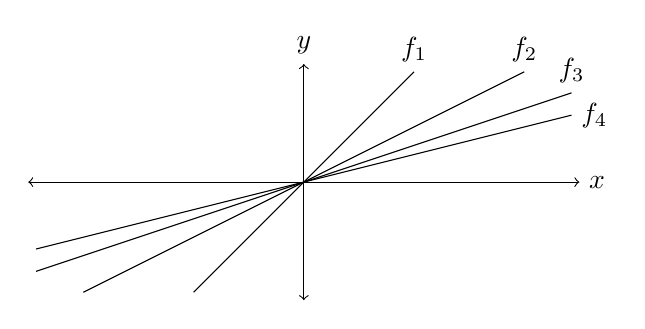
\begin{tikzpicture}
      \draw[<->] (-3.5, 0) -- (3.5, 0) node[right] {$x$};
      \draw[<->] (0, -1.5) -- (0, 1.5) node[above] {$y$};
      \draw[domain=-1.4:1.4, samples=2] plot({\x}, {\x}) node[above] {$f_1$};
      \draw[domain=-2.8:2.8, samples=2] plot({\x}, {\x/2}) node[above] {$f_2$};
      \draw[domain=-3.4:3.4, samples=2] plot({\x}, {\x/3}) node[above] {$f_3$};
      \draw[domain=-3.4:3.4, samples=2] plot({\x}, {\x/4}) node[right] {$f_4$};
    \end{tikzpicture}
  \end{center}
and the functions are converging ``pointwise'' to the constant function
$f(x)=0$. Next consider the functions $f_n$ defined on $[0,\infty)$ where\\\\
\begin{minipage}{0.4\textwidth}
  $$f_n=\begin{cases}
    x^n & x\in[0,1] \\
    1 & x\in(1,\infty)
  \end{cases}$$
\end{minipage}
\begin{minipage}{0.6\textwidth}
  \begin{center}
    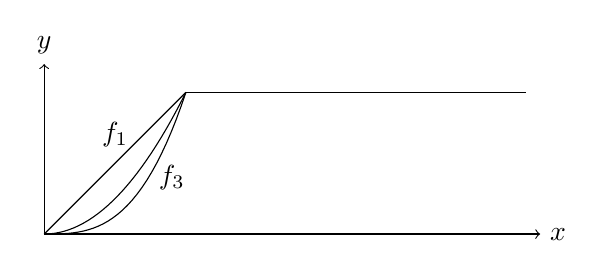
\begin{tikzpicture}[scale=1.8]
      \draw[->] (0, 0) -- (3.5, 0) node[right] {$x$};
      \draw[->] (0, 0) -- (0, 1.2) node[above] {$y$};
      \draw[domain=0:1, samples=2] plot({\x}, {\x});
      \draw[domain=0:1, samples=30] plot({\x}, {\x^2});
      \draw[domain=0:1, samples=30] plot({\x}, {\x^3});
      \draw[domain=1:3.4, samples=2] plot({\x}, {1});
      \node at (0.5,0.7) {$f_1$};
      \node at (0.9,0.4) {$f_3$};
    \end{tikzpicture}
  \end{center}
\end{minipage}\\\\
The picture here is as shown and the limit approaches a function resembling a
step. In this, each $f_n$ is continuous, but the pointwise limit is not
continuous.

\begin{defi}
  A sequence of functions $\{f_n\}$ \define{converges uniformly} to a function
  $f$ if for every $\epsilon>0$ there is an integer $N$ such that $m\ge N$
  implies $|f_n(x)-f(x)|\le\epsilon$ for all $x\in E$.
\end{defi}

\begin{prop}[Cauchy Criterion]
  The sequence $\{f_n\}$ converges uniformly if and only if for every
  $\epsilon>0$ there exists an integer $N$ such that $n\ge N$ and $m\ge N$
  implies $|f_n(x)-f_m(x)|\le\epsilon$ for all $x\in E$.
\end{prop}

\begin{thm}
  Suppose $f_n\to f$ uniformly on a set $E$ in a metric space. Let $x$ be a
  limit point of $E$ and suppose $\lim_{t\to x}f_n(t)=A_n$ ($n=1,2,3,\ldots$).
  Then $\{A_n\}$ converges and $\lim_{t\to x}f(t)=\lim_{n\to\infty}A_n$. In
  other words,
  $$\lim_{t\to x}\lim_{n\to\infty}f_n(t)=\lim_{n\to\infty}\lim_{t\to x}f_n(t)$$
\end{thm}

\begin{pf}
  Let $\epsilon>0$. By the uniform convergence of $\{f_n\}$, there exists an
  $N$ such that $n\ge N$, $m\ge N$, $t\in E$ imply
  $|f_n(t)-f_m(t)|\le\epsilon$. Letting $t\to x$ yields $|A_n-A_m|\le\epsilon$
  when $n\ge N$ and $m\ge M$, showing that $\{A_n\}$ is a Cauchy sequence (of
  complex numbers) and therefore converges to some $A$. Note that for $n\in\NN$
  and $t\in E$,
  $$|f(t)-A|\le|f(t)-f_n(t)|+|f_n(t)-A_n|+|A_n-A|$$
  by the Triangle Inequality. Now choose $n$ such that for all $t\in E$,
  $|f(t)-f_n(t)|\le\frac{\epsilon}{3}$ (which we can do since $f_n\to f$
  uniformly) and such that $|A_n-A|\le\frac{\epsilon}{3}$. Then for this $n$,
  choose a neighborhood $V$ of $x$ such that
  $|f_n(t)-A_n|\le\frac{\epsilon}{3}$ when $t\in V\cap E$, $t\neq x$. It
  follows that $|f(t)-A|\le\epsilon$ when $t\in V\cap E$, $t\neq x$, which is
  equivalent to $\lim_{t\to x}f(t)=\lim_{n\to\infty}A_n$.
\end{pf}

\begin{cor}
  If $\{f_n\}$ is a sequence of continuous functions, and if $f_n\to f$
  uniformly, then $f$ is continuous.
\end{cor}

\begin{pf}
  By the previous theorem, $\lim_{t\to x}f_n(t)=A_n=f_n(x)$ and $\lim_{t\to
  x}f(t)=\lim_{n\to\infty}A_n=\lim_{n\to\infty}f_n(x)=f(x)$.
\end{pf}

\begin{defi}
  If $X$ is a metric space, then $\SC(X)$ denotes the set of all continuous,
  complex-valued, and bounded functions with domain $X$.
\end{defi}

\begin{defi}
  We can associate to each $f\in\SC(X)$ its \define{supremum norm}
  $$\|f\|=\sup_{x\in X}|f(x)|$$
\end{defi}

\begin{prop}
  Suppose $f,g\in\SC(X)$.
  \begin{enumerate}
    \item $\|f\|<\infty$.
    \item $\|f\|=0$ if and only if $f$ is the zero function.
    \item $\|f+g\|\le\|f\|+\|g\|$.
  \end{enumerate}
\end{prop}

\begin{prop}
  Define the distance between $f$ and $g$ to be $\|f-g\|$. Then $\SC(X)$ is a
  metric space.
\end{prop}

\begin{prop}
  A sequence $\{f_n\}$ converges to $f$ in $\SC(X)$ if and only if $f_n\to f$
  uniformly on $X$.
\end{prop}

\begin{prop}
  The above metric makes $\SC(X)$ into a complete metric space.
\end{prop}

\begin{pf}
  Suppose $\{f_n\}$ is a Cauchy sequence in $\SC(X)$. Thus for every
  $\epsilon>0$, there is an $N$ such that $\|f_n-f_m\|<\epsilon$ whenever $n\ge
  N$ and $m\ge N$. Thus there is a function $f:X\to\CC$ to which $\{f_n\}$
  converges uniformly. Thus $f$ is continuous. Also, $f$ is bounded since there
  is an $n$ such that $|f(x)-f_n(x)|<1$ for all $x\in X$ and $f_n$ is bounded.
  Hence $f\in\SC(X)$ and since $f_n\to f$ uniformly on $X$, we have
  $\|f-f_n\|\to0$ as $n\to\infty$.
\end{pf}

\begin{thm}[Stone-Weierstrass Theorem]
  If $f$ is a continuous complex function on $[a,b]$, then there exists a
  sequence of polynomials $\{P_n\}$ such that $\lim_{n\to\infty}P_n(x)=f(x)$
  uniformly on $[a,b]$. Furthermore, if $f$ is real, then $P_n$ can be taken to
  be real.
\end{thm}

\end{document}
